\section{Product perspective}
\label{sec:product_perspective}%



\subsection{Scenarios}
\label{subsec:scenarios}%
\begin{itemize}
    \item \textbf{Scenario 1 : Companies Submit Internship Postings}
TechCorp, a fast-growing software company, wants to attract top talent for its upcoming AI project. HR manager Alex logs into the platform, fills out a detailed form including roles such as "AI Research Intern," qualifications like "Python and machine learning basics," and perks like a monthly stipend. Alex sets the application deadline and hits "Publish," making the internship visible to thousands of aspiring developers. 
Alex can also modify details about the internship in order to better clarify information or make the offer more appealing to developers.

    \item \textbf{Scenario 2 : Students Create Profiles and Upload CVs}
Emma, a computer science student, registers on the platform after her professor’s recommendation. She proceeds by uploading her updated CV, enhanced thanks to the help of he platform, highlighting her achievements, such as winning a hackathon, and finally she gives her preferences for internships. The system then auto-generates a sleek profile for her, ensuring she stands out when companies view her application. 

    \item \textbf{Scenario 3 : Students Browse and Apply for Internships} 
Carlos, a final-year engineering student, dreams of working in the renewable energy sector. He logs into the internship platform and clicks on “Browse Internships.” Using the filters provided, he specifies his preferences: roles related to renewable energy, locations within Europe, and remote options.
The platform then shows him a selected list of opportunities. One particular posting catches his eye: an internship at Solar Innovations, offering a role as an Energy Data Analyst. He clicks on the listing to read the details, which include a comprehensive description of the role, qualifications required, and benefits.
Excited about the opportunity, Carlos reviews his profile to ensure everything is up to date. With a click of the “Apply” button, Carlos submits his application.

    \item \textbf{Scenario 4 : \textbf{System Recommends Internships to Students} }
Jane, a computer science student, logs into the platform but feels overwhelmed by the number of postings. Uncertain of what to do, she enters the “Recommended for You” section. Here, the platform uses her profile information, like her skills, past internships, and preferences, to suggest a set of internships that best fit to her career goals. 

\item \textbf{Scenario 5 : \textbf{Companies Receive and Review Applications} }
At TechApps, Sophia logs into the company dashboard to review applications for the UI/UX intern position. The system presents the list of candidates that applied for the internship, each accompanied by a profile summary. Sophia filters and ranks applications based on the required skills and qualifications.
Jane’s application catches her attention so she adds her to the shortlist and schedules an interview, leaving a note: “Potential strong fit—verify design process knowledge in the interview.”

\item \textbf{Scenario 6 :\textbf{Interview Scheduling and Management}}
Jane is thrilled to receive an email from TechApps inviting her to an interview. The email provides a link to the platform, where she can view available time slots. Jane selects a convenient slot for the interview. The platform confirms the booking and sends her and Sophia a notification, ensuring they won’t forget the appointment. On the day of the interview, both Jane and Sophia receive a reminder email with a link to the video meeting. Jane logs in 10 minutes early to prepare. The interview runs smoothly, as the system assists both Jane and Sophia by providing access to Jane’s profile and portfolio during their discussion.

\item \textbf{Scenario 7 : Feedback Collection:} 
After the interview, Sophia logs into the company dashboard to provide feedback on Jane’s application. She rates Jane highly for her design skills but notes that she could improve her knowledge of user-centered design principles. Sophia’s comments are saved in the system and shared with Jane as constructive feedback. Meanwhile, Jane also leaves feedback on her experience with TechApps, praising the structured interview process and mentioning how the questions helped her reflect on her skills. Both sets of feedback contribute to improving the system’s recommendations for future interactions.
 
\item \textbf{Scenario 8 : \textbf{Internship Monitoring by Universities} }
Professor Adams oversees the internships of students from his university. He logs into the platform and accesses the “Internship Monitoring” dashboard. He sees that Jane has started her internship at TechApps and reviews the company’s details and the role description to ensure it aligns with the university’s educational standards. Professor Adams can view Jane’s progress reports and sends her a message: “Jane, I noticed your internship involves user research. Please ensure you document your findings, as we can integrate them into your coursework next semester.”

\item \textbf{Scenario 9 : \textbf{Complaint Handling}}
A few weeks into her internship, Jane feels uncertain about the expectations for her role. She uses the platform’s complaint system to raise a concern. A university representative reviews her complaint and contacts both Jane and her supervisor at TechApps. After a mediated discussion, the supervisor provides Jane with a clearer outline of her responsibilities. Jane is relieved, and the improved communication ensures the internship continues smoothly. The entire process is recorded and saved by the system for future reference.

\item \textbf{Scenario 10 : \textbf{System Updates Recommendations} }
Based on feedback collected from Jane and other users, the platform updates its recommendation algorithms. It notices that students like Jane, who excel in design but lack industry exposure, benefit most from internships that focus on mentorship and practical application. The system adjusts its filters to prioritize such opportunities for students with similar profiles, enhancing the relevance of its recommendations.

\item \textbf{Scenario 11 : \textbf{Post-Internship Evaluation} }
At the end of her internship, Jane and her supervisor complete post-internship evaluations on the platform. Jane rates the company highly for its supportive environment, while her supervisor highlights her strengths in creativity and adaptability. These evaluations are stored in the system, contributing to its database for improving internship matchmaking. Jane’s positive feedback also boosts TechApps’ visibility on the platform.

\item \textbf{Scenario 12 : Statistical Data Analysis} 
The platform’s analytics team compiles data on completed internships. They identify trends, such as the success rate of students in different industries and the feedback ratings for various companies.
Universities use this data to adjust their curricula, ensuring students are better prepared for internships. Companies like TechApps also analyze their feedback to improve their on boarding processes.

\item \textbf{Scenario 13 : Notifications and Alerts} 
Jane is now in her final semester, actively seeking full-time roles. The platform sends her regular notifications about new internship opportunities, application deadlines, and interview reminders. These alerts keep Jane engaged and ensure she doesn’t miss out on any chance to enhance her career. 


\end{itemize}
\subsection{Class Diagrams}
\label{subsec:class_diagrams}%
\begin{figure}[H]
    \centering
    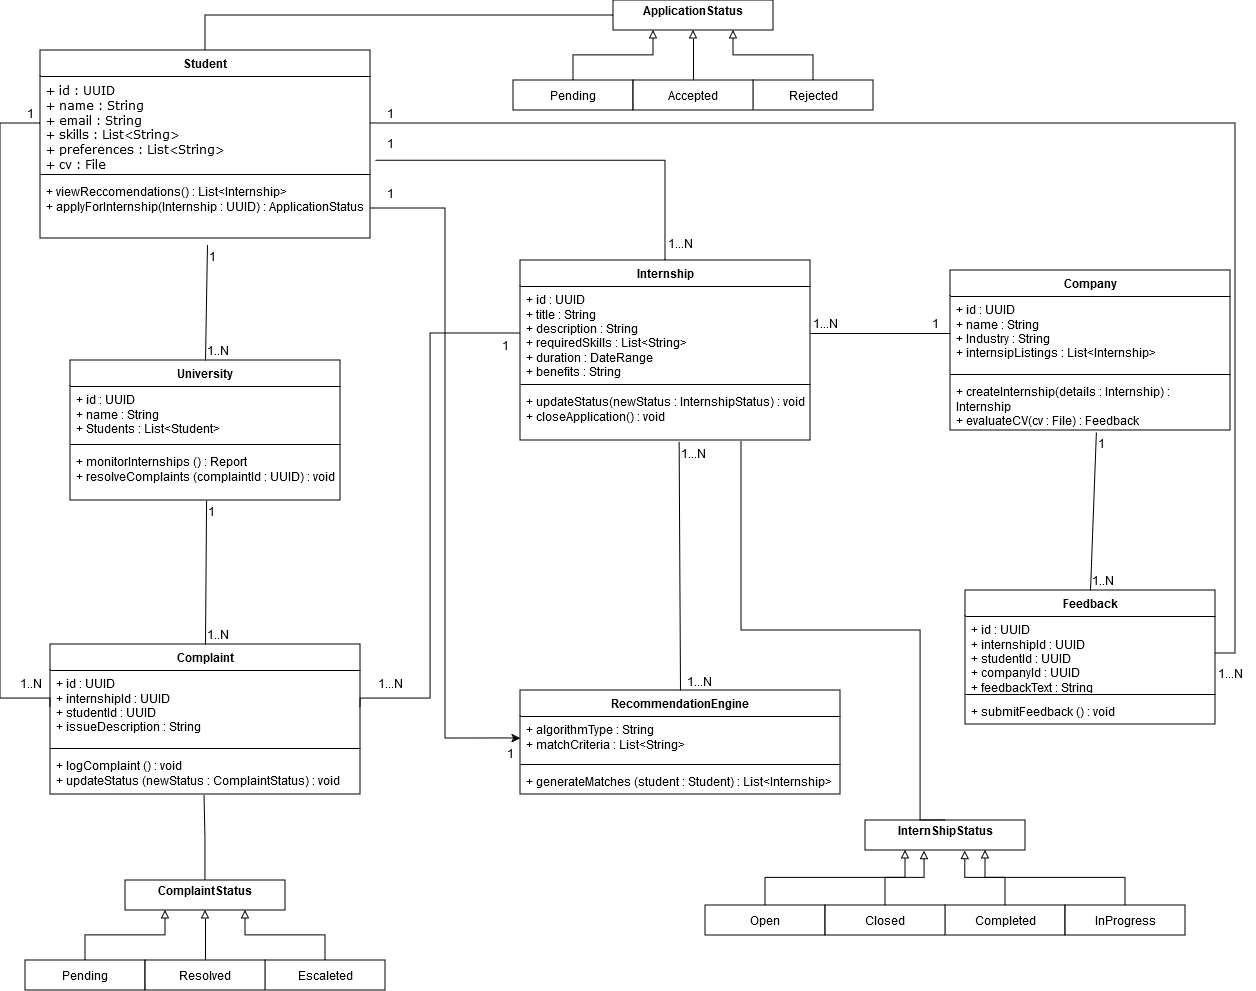
\includegraphics[width=1\linewidth]{Images/Class diagrams/ClassDiagram.png}
    \caption{Class Diagram}
    \label{fig:enter-label}
    
    
\end{figure}

\subsection{State Diagrams}
\label{subsec:class_diagrams}%

\paragraph{Sign-up} Initially, users can create a generic account that allows them to browse available posts without the ability to post. To upgrade to a full account, they must verify their email address, select a role (either as a student or a company), and complete the required fields for their chosen role.

\begin{figure}[H]
    \centering
    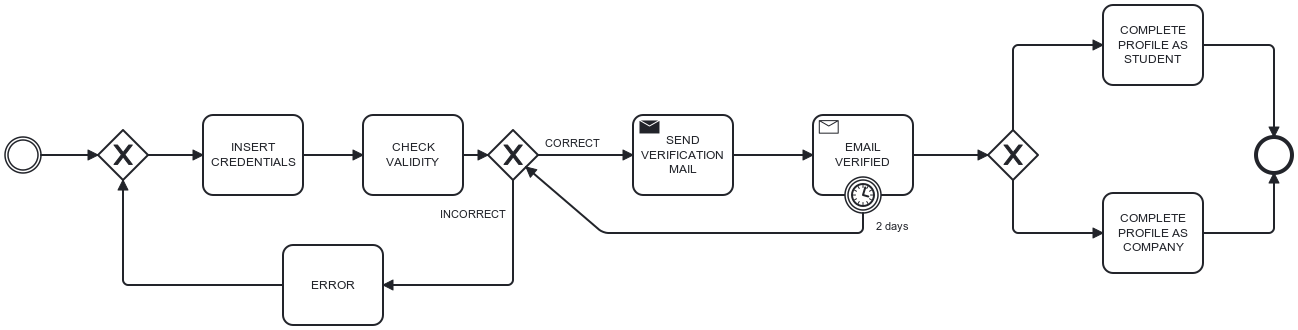
\includegraphics[width=1\linewidth]{Images//state diagrams/SIGNUP.png}
    \caption{Sign-up state diagram}
    \label{fig:enter-label}
\end{figure}

\paragraph{Login} During login, the system verifies the user's credentials to ensure they are correct. Upon successful authentication, the user is redirected to their personalized homepage.

\begin{figure}[H]
    \centering
    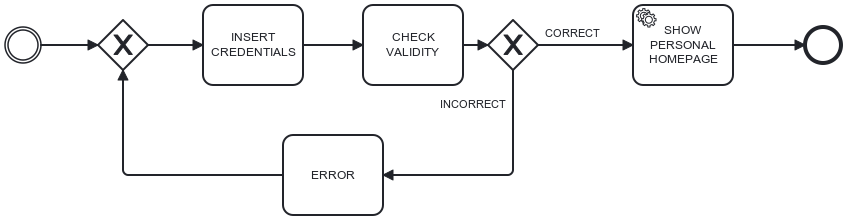
\includegraphics[width=1\linewidth]{Images//state diagrams/LOGIN.png}
    \caption{Login state diagram}
    \label{fig:enter-label}
\end{figure}

\paragraph{Apply for an internship} The student reviews their recommended internships. If they decide to apply for one, they must contact the company, which will proceed to schedule an interview. If the interview is successful and both parties agree, the internship will be communicated to the university.

\begin{figure}[H]
    \centering
    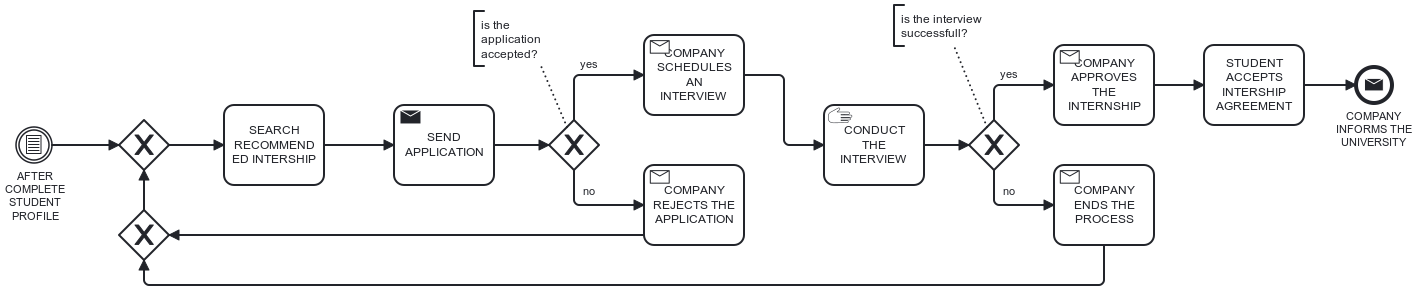
\includegraphics[width=1\linewidth]{Images//state diagrams/APPLICATION.png}
    \caption{Application state diagram}
    \label{fig:enter-label}
\end{figure}

\paragraph{Complaints handling} Both students and companies can submit a complaint during the internship. The university evaluates the complaint to determine whether intervention is necessary. If no intervention is required, the process ends without further action. However, if intervention is necessary, the university attempts to mediate between the parties to resolve the issue. If mediation is successful, the process concludes, and the internship continues as usual. On the other hand, if mediation fails or the issue remains unresolved, the university decides to terminate the internship. Before finalizing the termination, the university ensures that both parties are informed about the decision.

\begin{figure}[H]
    \centering
    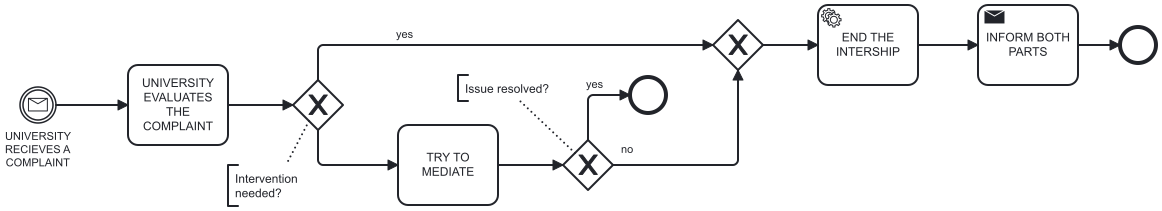
\includegraphics[width=1\linewidth]{Images//state diagrams/COMPLAINTS.png}
    \caption{Complaint diagram}
    \label{fig:enter-label}
\end{figure}

\section{Product functions}
\label{sec:product_functions}%

Here's the main functions of S\&C system:

\paragraph{Register to the platform}
The S\&C platform allows user to register, providing username and password. While registering to the system, users must first declare that they have read and understood the Privacy Statement. They are also required to accept the Terms and Conditions, which request consent for the acquisition and processing of their personal data for the purpose of using the platform's matching analysis and statistics.

\paragraph{Upgrade to Student account}
The S\&C platform allows students to register. During the registration process, users are required to provide the following information:
\begin{center}
\renewcommand{\arraystretch}{1}
\begin{tabular}{|p{5cm}|p{5cm}|}
\hline
\textbf{Field}  & \textbf{Note} \\
\hline
Full name &  \\
\hline
Password & Security standards check\\
\hline
Academic email address & Checking an existing university domain \\
\hline
Attending university & automatically populated field \\
\hline
Phone number &  \\
\hline
Postal Code & Matching parameter \\
\hline
\end{tabular}
\end{center}

\paragraph{Upgrade to Company account}
The S\&C platform allows companies to register. During the registration process, users are required to provide the following information:
\begin{center}
\renewcommand{\arraystretch}{1}
\begin{tabular}{|p{5cm}|p{5cm}|}
\hline
\textbf{Field} & \textbf{Notes} \\
\hline
Full name &  \\
\hline
Password & Checking security standards \\
\hline
Office address & Matching parameter \\
\hline
Office phone number & Optional \\
\hline
\end{tabular}
\end{center}

\paragraph{Post an internship}A button within the company's dashboard that opens a form for creating and submitting a new internship posting, including fields for job title, description, requirements, salary, and duration

\paragraph{Check recommended internships}A searchable and filterable page accessible to all users, displaying a list of internships with brief descriptions and company details.
\paragraph{Apply for an internship}A button on each internship's detail page that triggers a form submission, allowing students to send their application with a personalized message and resume upload.
\paragraph{Evaluate an application}A company dashboard feature showing a list of received applications with applicant details, resumes, and the option to accept, reject, or schedule interviews.
\paragraph{Schedule an interview}An action available on an application detail page that opens a scheduling form, allowing the company to set the interview's date, time, and mode.
\paragraph{Submit a complaint}A button in the dashboard (available to students and companies) that opens a form for submitting a formal complaint, including issue details.
\paragraph{Submit a feedback}A post-internship form accessible to both students and companies where they can rate the experience, provide comments, and suggest improvements for future internships.

\section{User characteristics}
\label{sec:user_characteristics}%

The actors of the application are the following:

\begin{itemize}
    \item \textbf{Registered User}: A single person registered in the platform before selecting their role (Student or company). This type of user has limited access to the platform: they can browse published internships to view basic information, but they cannot interact with them. To unlock advanced features, the user must complete the registration process by selecting their role.
    \item \textbf{Student}: A single person registered as a student on the platform. Their aim is to find internships aligned with their academic background, skills, and career goals. They need only an active account, an internet connection, and access to a digital CV.
    \item \textbf{Company}: An organization of people registered on the platform. Its goal is to publish internship opportunities, examine applications, and hire suitable candidates. It requires an active account, an internet connection, and major internship details.
    \item \textbf{University}: A career services representative with a passive role on the platform. Universities are contacted only if an internship goes wrong or complaints emerge from companies or students. Their task is to review the situation and, if necessary, interrupt the internship. They need access to relevant student and company data.
\end{itemize}

\section{Assumptions, dependencies and constraints}
\label{sec:assumptions_dependencies_and_constraints}%
\newcounter{da} 
\setcounter{da}{1}
\newcommand{\cda}{D\arabic{da}\stepcounter{da}} 
\begin{center}
    \renewcommand{\arraystretch}{2}
    \begin{longtable}{ l p{0.8\linewidth} } 
        \hline
        \textbf{ID} & \textbf{Description} \\ 
        \hline
        \cda & Internship descriptions are comprehensive and reliable \\ \hline
        \cda & CVs accurately reflect students' skills and experiences \\ \hline
        \cda & Universities actively oversee internships and intervene when necessary \\ \hline
        \cda & Companies manage interview timelines and conduct them professionally \\ \hline
        \cda & Users provide meaningful feedback to improve the system \\ \hline
        \cda & Problems are reported in a timely manner by all parties \\ \hline
        \cda & The platform supports high user traffic without performance issues \\ \hline
        \caption{Domain Assumptions.}
        \label{tab:worldph_tab}%
    \end{longtable}
\end{center}

